% Candidate source: src-cb0092e0533abc5b37a4e6843ba9688dfd851d0597a8dd9d44a827bd35e58290
% Source PDF SHA-256: 4ffc26d1ee893834e7cdf6a1b6ab3385fb97dd791d838d2630538461026ca7ad
% PDF page 2 (printed page 201), question 21.
% Redraw follows visible/hidden edges; perspective is schematic, not to scale.
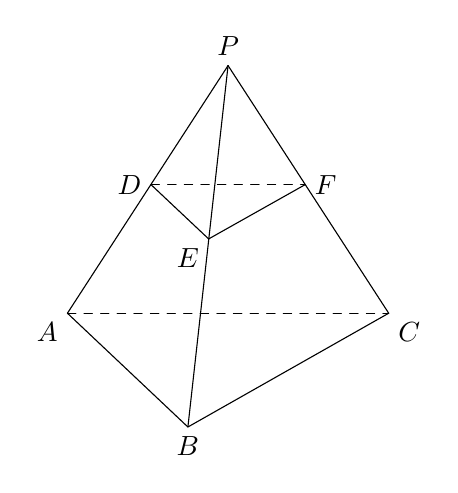
\begin{tikzpicture}[line cap=round,line join=round,x=0.85cm,y=0.85cm]
  \coordinate (P) at (2.4,4.2);
  \coordinate (A) at (0,0.5);
  \coordinate (B) at (1.8,-1.2);
  \coordinate (C) at (4.8,0.5);

  % Points on lateral edges for section DEF
  \coordinate (D) at (1.25,2.42);
  \coordinate (E) at (2.11,1.61);
  \coordinate (F) at (3.55,2.42);

  % Hidden edges (back edges)
  \draw[dashed] (A) -- (C);
  \draw[dashed] (D) -- (F);

  % Visible edges: pyramid lateral edges
  \draw (P) -- (A);
  \draw (P) -- (B);
  \draw (P) -- (C);

  % Base front edges
  \draw (A) -- (B) -- (C);

  % Section front edges
  \draw (D) -- (E) -- (F);

  % Labels
  \node[above] at (P) {$P$};
  \node[left] at (D) {$D$};
  \node[below left] at (E) {$E$};
  \node[right] at (F) {$F$};
  \node[below left] at (A) {$A$};
  \node[below] at (B) {$B$};
  \node[below right] at (C) {$C$};
\end{tikzpicture}
